\documentclass{beamer}\usepackage[]{graphicx}\usepackage[]{color}
%% maxwidth is the original width if it is less than linewidth
%% otherwise use linewidth (to make sure the graphics do not exceed the margin)
\makeatletter
\def\maxwidth{ %
  \ifdim\Gin@nat@width>\linewidth
    \linewidth
  \else
    \Gin@nat@width
  \fi
}
\makeatother

\definecolor{fgcolor}{rgb}{0.345, 0.345, 0.345}
\newcommand{\hlnum}[1]{\textcolor[rgb]{0.686,0.059,0.569}{#1}}%
\newcommand{\hlstr}[1]{\textcolor[rgb]{0.192,0.494,0.8}{#1}}%
\newcommand{\hlcom}[1]{\textcolor[rgb]{0.678,0.584,0.686}{\textit{#1}}}%
\newcommand{\hlopt}[1]{\textcolor[rgb]{0,0,0}{#1}}%
\newcommand{\hlstd}[1]{\textcolor[rgb]{0.345,0.345,0.345}{#1}}%
\newcommand{\hlkwa}[1]{\textcolor[rgb]{0.161,0.373,0.58}{\textbf{#1}}}%
\newcommand{\hlkwb}[1]{\textcolor[rgb]{0.69,0.353,0.396}{#1}}%
\newcommand{\hlkwc}[1]{\textcolor[rgb]{0.333,0.667,0.333}{#1}}%
\newcommand{\hlkwd}[1]{\textcolor[rgb]{0.737,0.353,0.396}{\textbf{#1}}}%
\let\hlipl\hlkwb

\usepackage{framed}
\makeatletter
\newenvironment{kframe}{%
 \def\at@end@of@kframe{}%
 \ifinner\ifhmode%
  \def\at@end@of@kframe{\end{minipage}}%
  \begin{minipage}{\columnwidth}%
 \fi\fi%
 \def\FrameCommand##1{\hskip\@totalleftmargin \hskip-\fboxsep
 \colorbox{shadecolor}{##1}\hskip-\fboxsep
     % There is no \\@totalrightmargin, so:
     \hskip-\linewidth \hskip-\@totalleftmargin \hskip\columnwidth}%
 \MakeFramed {\advance\hsize-\width
   \@totalleftmargin\z@ \linewidth\hsize
   \@setminipage}}%
 {\par\unskip\endMakeFramed%
 \at@end@of@kframe}
\makeatother

\definecolor{shadecolor}{rgb}{.97, .97, .97}
\definecolor{messagecolor}{rgb}{0, 0, 0}
\definecolor{warningcolor}{rgb}{1, 0, 1}
\definecolor{errorcolor}{rgb}{1, 0, 0}
\newenvironment{knitrout}{}{} % an empty environment to be redefined in TeX

\usepackage{alltt}


\usepackage{alltt}%
\usetheme{Boadilla}
\usecolortheme{seahorse}

%\usepackage{listings}
\makeatletter
\def\maxwidth{ %
  \ifdim\Gin@nat@width>\linewidth
    \linewidth
  \else
    \Gin@nat@width
  \fi
}
\makeatother

\usepackage[utf8]{inputenc}
\usepackage{default}

\usepackage{xcolor}%for color mixing

\usepackage{amsmath}%
\usepackage{amsfonts}%
\usepackage{amssymb}%
\usepackage{graphicx}

\usepackage{tikz}
\usepackage{multirow}
\usepackage{booktabs}

\setbeamertemplate{itemize/enumerate body begin}{\small}

%%%%%%%%%%%%%%%%%%%%%%%%%%%%%%%%%%%%%%%%%%%%%%%%%%%%%%%%%%%%%%%%%%%%%%%%%%%%%%%%%%

\title[Logistic regression]{Generalized linear models and the logistic regression}
\author{Timoth\'ee Bonnet}
\institute{Thanks to BDSI for support!}
\date{\today}
\IfFileExists{upquote.sty}{\usepackage{upquote}}{}
\begin{document}

%\lstset{language=R}%code

\AtBeginSection[]
{
  \begin{frame}<beamer>
    \frametitle{}
    \tableofcontents[currentsection,sectionstyle=show/show,subsectionstyle=show/shaded/hide]% down vote\tableofcontents[currentsection,currentsubsection,hideothersubsections,sectionstyle=show/hide,subsectionstyle=show/shaded/hide] 
  \end{frame}
}



\begin{frame}{logiwhat?}

From Wikipedia:
\begin{quote}
The function was named in 1844 by Pierre François Verhulst, who studied it in relation to population growth. The initial stage of growth is approximately exponential (geometric); then, as saturation begins, the growth slows to linear (arithmetic), and at maturity, growth stops. Verhulst did not explain the choice of the term ``logistic", but it is presumably in contrast to the logarithmic curve and by analogy with arithmetic and geometric. His growth model is preceded by a discussion of arithmetic growth and geometric growth, and thus "logistic growth" is presumably named by analogy, logistic being from Ancient Greek logistikós, a traditional division of Greek mathematics. The term is unrelated to the military and management term logistics.
\end{quote}

The ``logit" function/unit/transform comes from the contraction of \textbf{log}istic un\textbf{it}.

\end{frame}
%%%%%%%%%%%%%%%


\begin{frame}{}
\maketitle

\end{frame}
%%%%%%%%%%%%%%%%%%%%%%%

\begin{frame}[fragile]{A simple linear model}
\centering

  \textbf{{\color{purple}{Response}} = {\color{blue}{Intercept}} + {\color{red}{Slope}} $\times$ {\color{orange}{Predictor}} + {\color{gray}{Error}}} \\

\begin{knitrout}\small
\definecolor{shadecolor}{rgb}{0.843, 0.867, 0.922}\color{fgcolor}
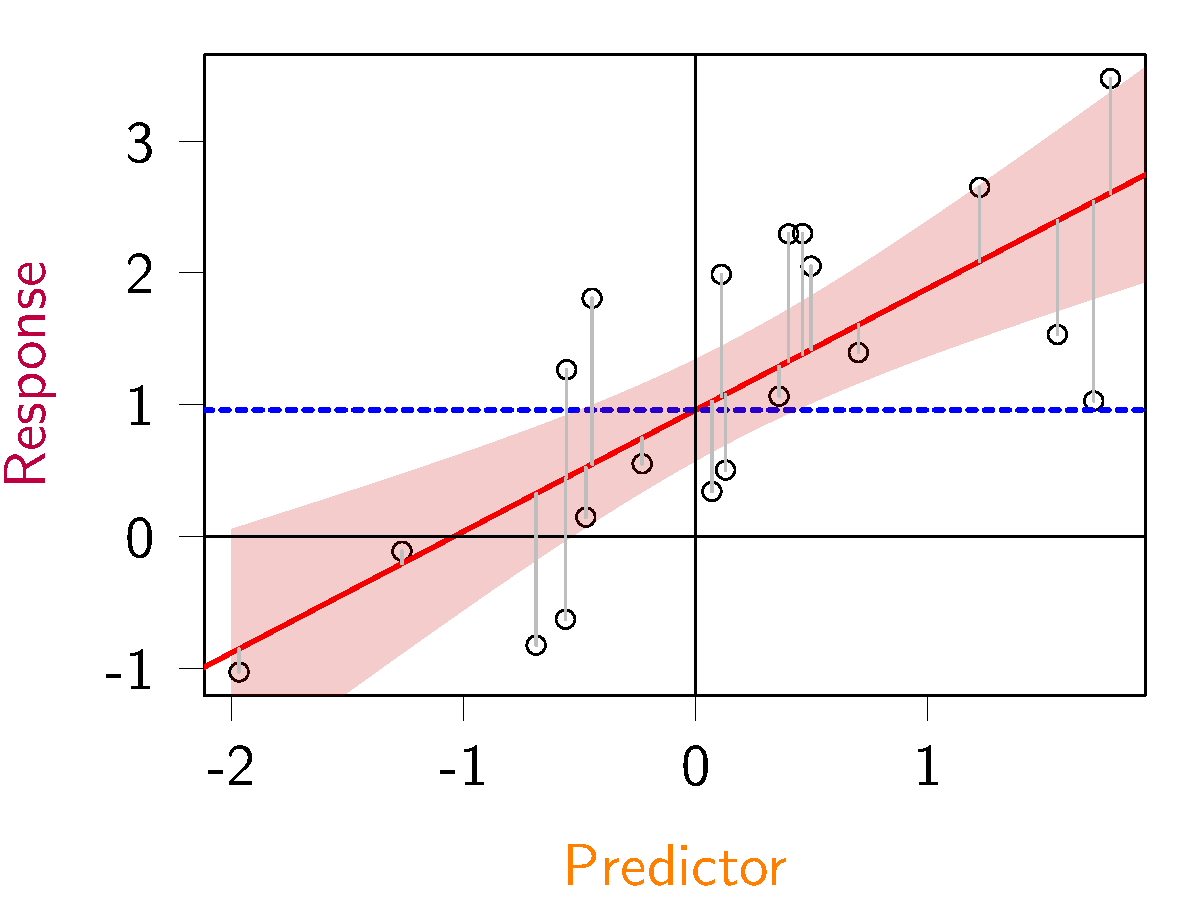
\includegraphics[width=0.8\textwidth,height=0.6\textwidth]{figure/lmprinc-1} 

\end{knitrout}
\end{frame}
%%%%%%%%%%%

\begin{frame}[fragile]{A simple linear model failure: binary data}
\centering

\begin{knitrout}\small
\definecolor{shadecolor}{rgb}{0.843, 0.867, 0.922}\color{fgcolor}
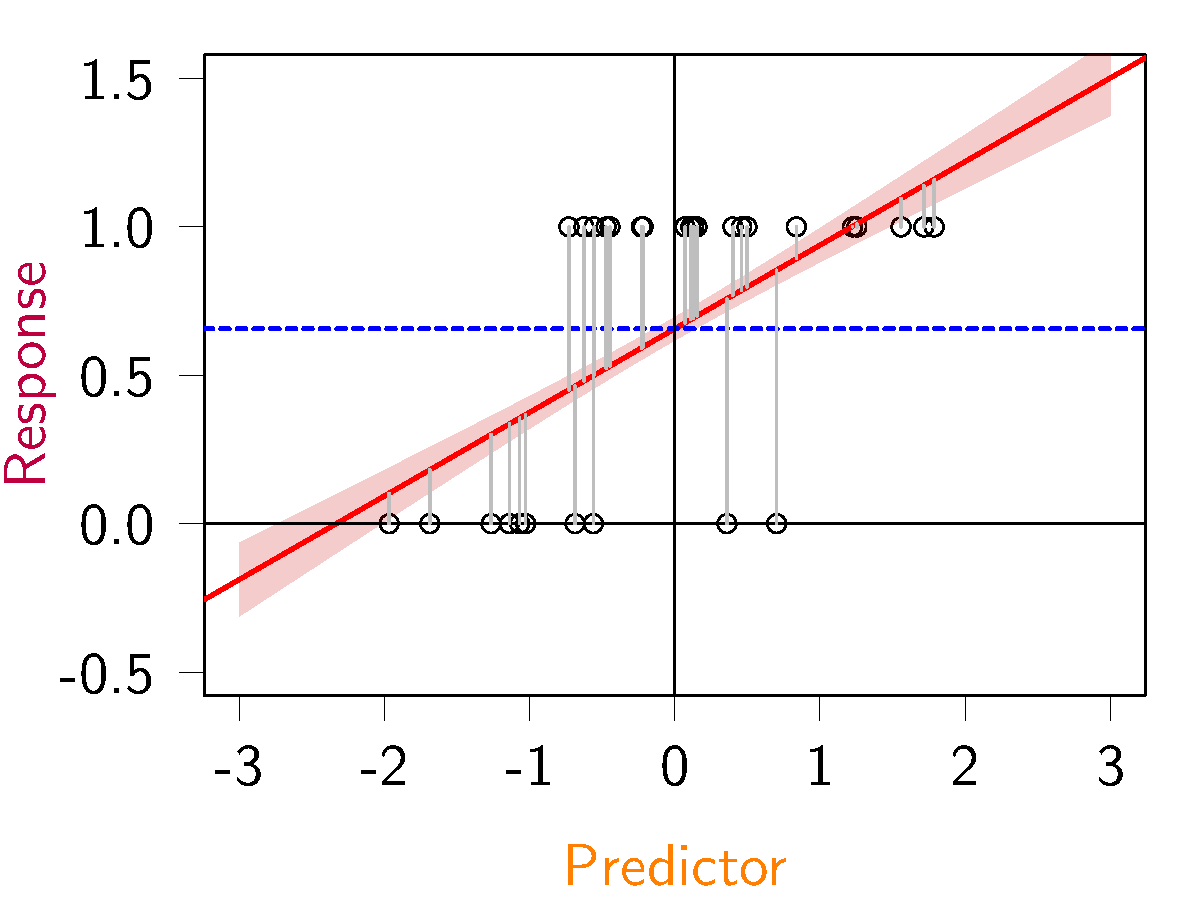
\includegraphics[width=0.8\textwidth,height=0.6\textwidth]{figure/binlmprinc-1} 

\end{knitrout}
  
\end{frame}
%%%%%%%%%%%

\begin{frame}{What we want our model to do}
\centering



\begin{knitrout}\small
\definecolor{shadecolor}{rgb}{0.843, 0.867, 0.922}\color{fgcolor}
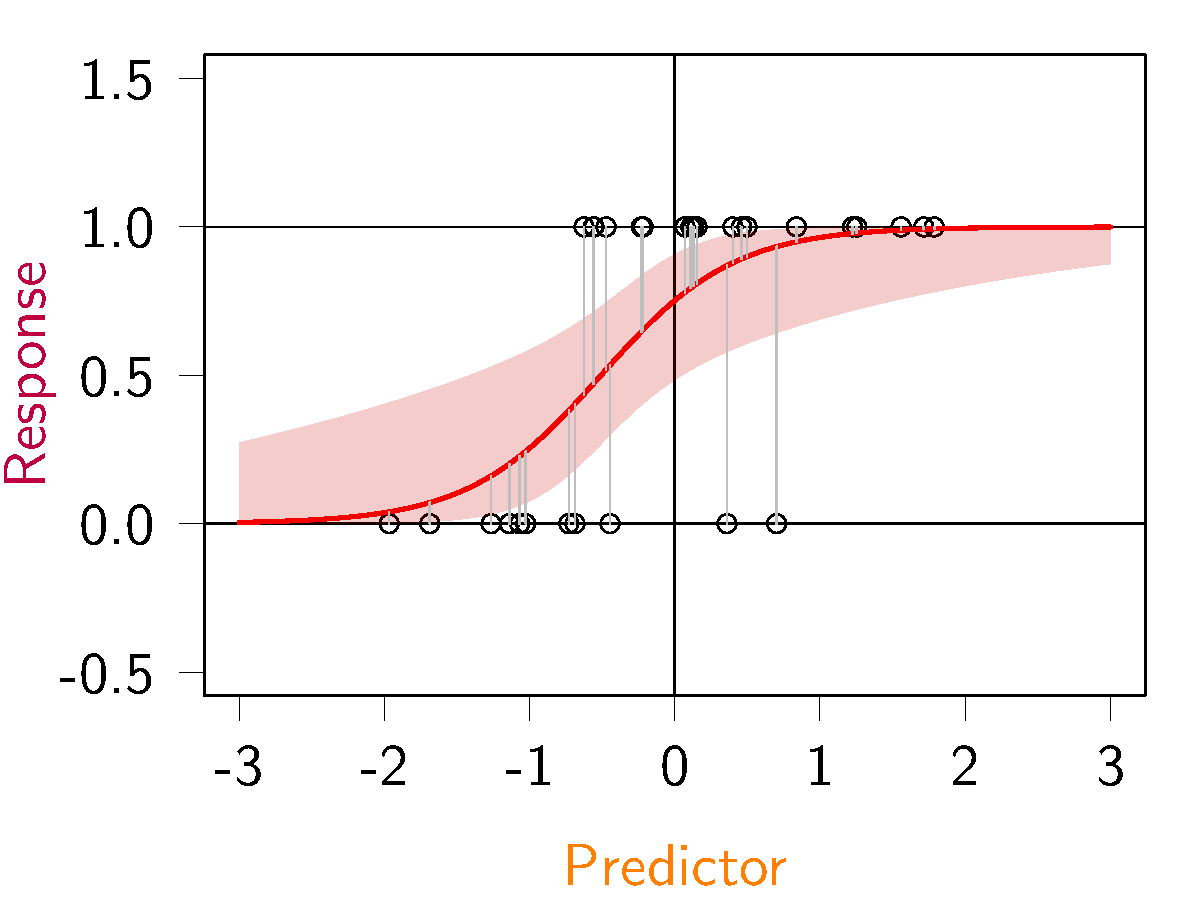
\includegraphics[width=0.8\textwidth,height=0.6\textwidth]{figure/logreg1-1} 

\end{knitrout}

\end{frame}
%%%%%%%%%%%%

\begin{frame}{What we want our model to do}
\centering
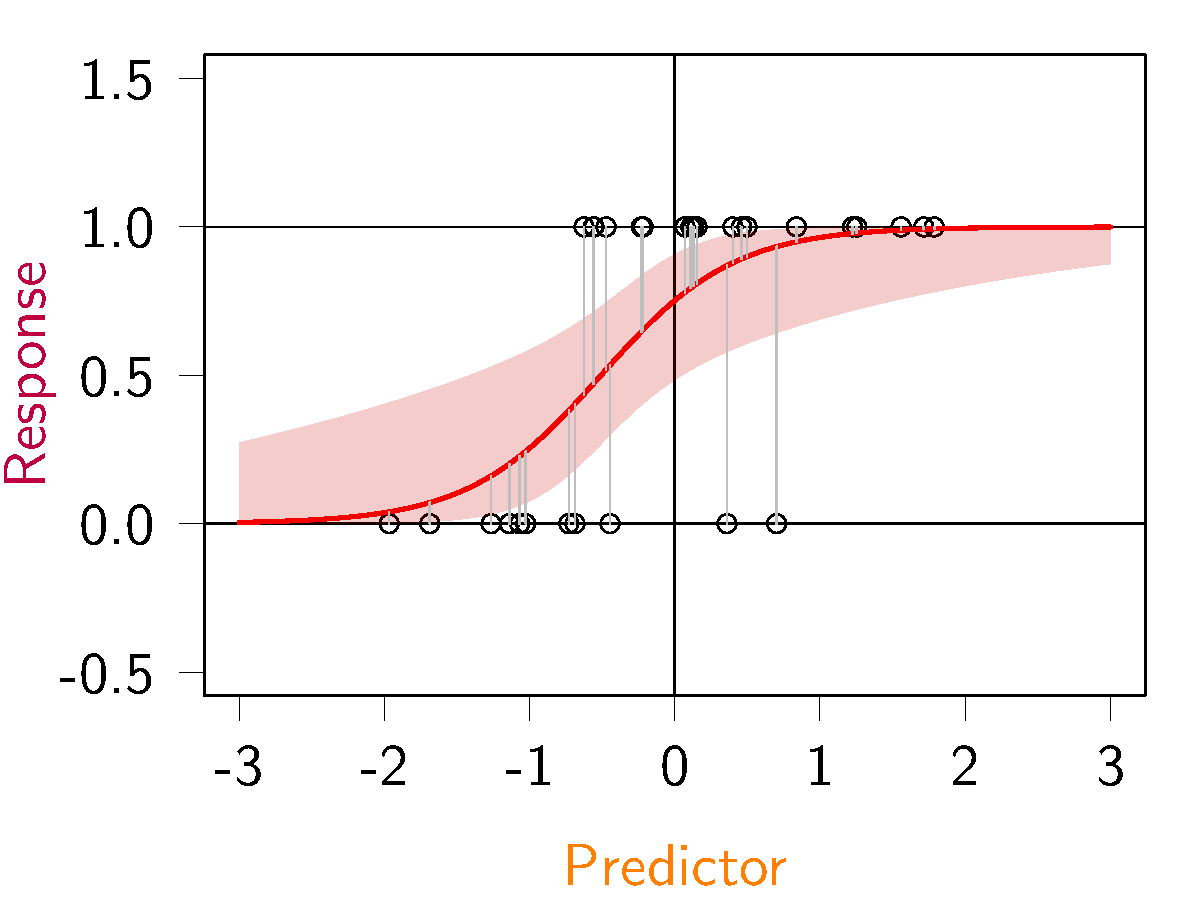
\includegraphics[width=0.5\textwidth]{figure/logreg1-1.pdf}

\begin{block}{What we need:}
  \begin{enumerate}[<+->]
    \item Convert the predictor open scale ($-\infty$ to $+\infty$) to a bounded scale (0 to 1)
    \item Acknowledge discrete data
    \item Response variability depends on expected value
  \end{enumerate}
\end{block}
\end{frame}
%%%%%%%%%%%

\begin{frame}{That is what a Generalized Linear Model does}

\begin{block}{Vocabulary warning}
  \begin{itemize}
    \item General Linear Model (=linear model with several responses, multivariate)
    \item \textbf{Generalized Linear Model (=non-normal errors, and uncertainty dependent on the mean)} 
  \end{itemize}
\end{block}

\pause

\begin{block}{What a GLM is:}
  \begin{enumerate}[<+->]
    \item \textbf{Linear function} (reponse = intercept + slope $\times$ predictor \dots)
    \item ``\textbf{Link function}" = a map between the linear function ($-\infty$ to $+\infty$) and a probability distribution (from 0 to 1 for Bernouilli)
    \item \textbf{Probability distribution} (Bernouilli, Binomial, Poisson\dots) thought to generate the data (either 0 or 1 for Bernouilli)
  \end{enumerate}
\pause[\thebeamerpauses]

GLMs fit continuous expected response; we observe discrete realizations
\end{block}

\end{frame}
%%%%%%%%%%%%%%%%%%%%%%%

\begin{frame}{What to do with logistic regression}
\centering
\only<1-2>{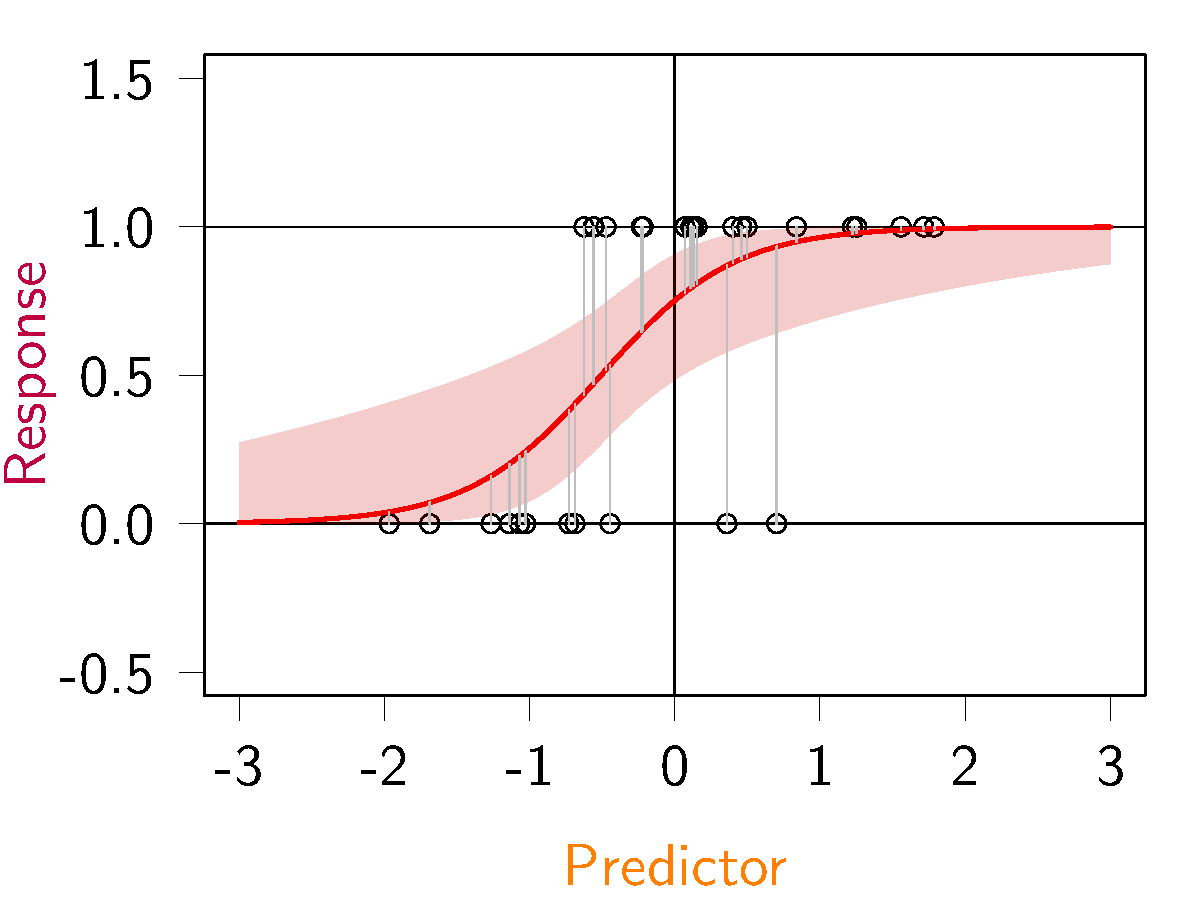
\includegraphics[width=0.5\textwidth]{figure/logreg1-1.pdf}}

\only<3>{
\begin{knitrout}\small
\definecolor{shadecolor}{rgb}{0.843, 0.867, 0.922}\color{fgcolor}
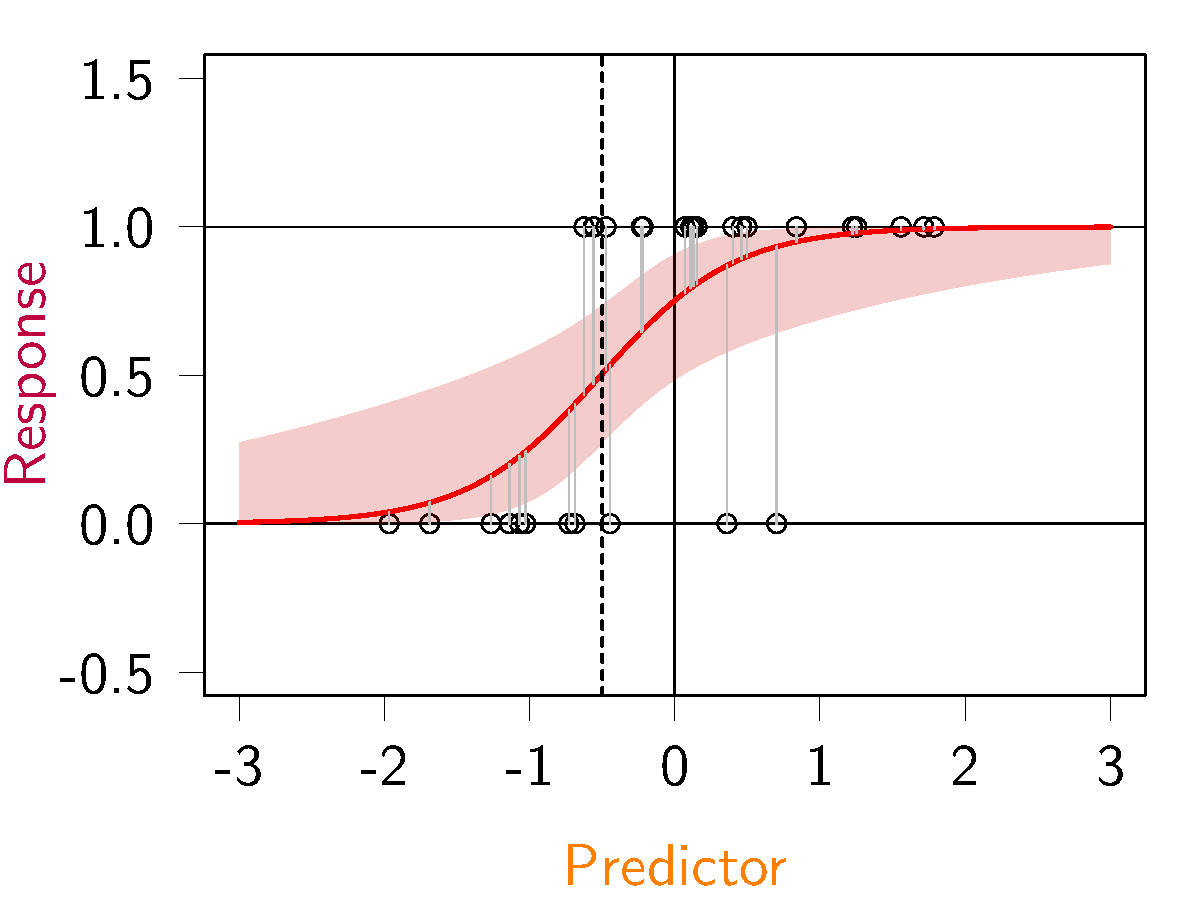
\includegraphics[width=0.5\textwidth,height=0.5\textheight]{figure/logreg2-1} 

\end{knitrout}
}

\only<4>{
\begin{knitrout}\small
\definecolor{shadecolor}{rgb}{0.843, 0.867, 0.922}\color{fgcolor}
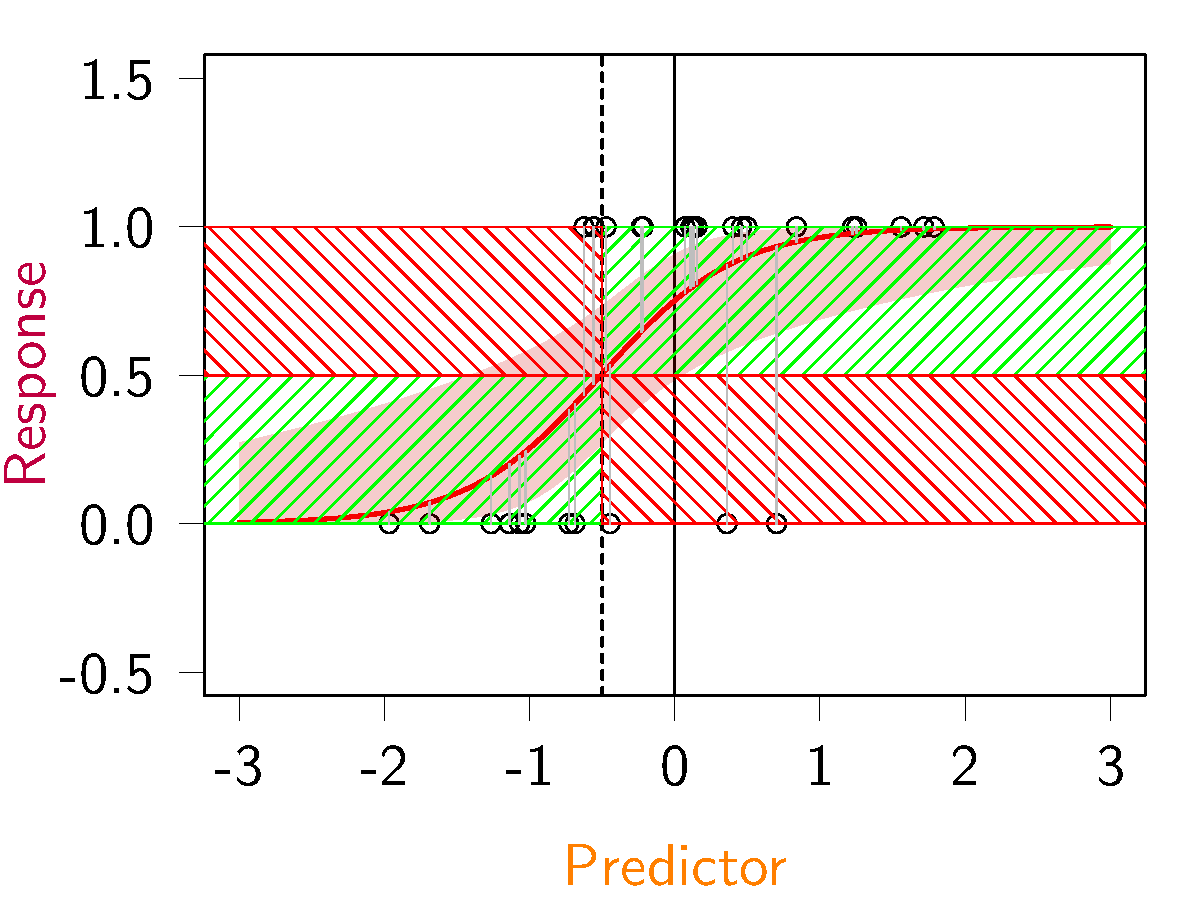
\includegraphics[width=0.5\textwidth,height=0.5\textheight]{figure/logreg3-1} 

\end{knitrout}
}

\begin{block}{}
\begin{enumerate}[<+->]
  \item Response increase/decrease with increasing predictor?
  \item Estimate probability of 0/1 given a predictor value
  \item Predict 0/1 and classify predictor values ($\rightarrow$ Machine Learning)
\end{enumerate}
\end{block}
\end{frame}
%%%%%%%%%%%%%%%%%%%%%%%

\begin{frame}{Exercise 1, fit a glm}

Load the dataset \texttt{survivalsize.csv}. It contains fake data of individual-based measurements of body size and of survival from the time of measurement to the next year. Look at a summary of the data and plot them. Do you think size affects survival?
Use the function glm() to fit a logistic regression. What should the \texttt{family} argument be? What is the direction of the effect of size on survival?

\end{frame}
%%%%%%%%%%%%%%%%%%%%%%%

\begin{frame}{Exercise 2, Model assumptions?}

In R some model assumptions of linear models are routinely checked using plot(lm()): residual normality, independance and homogeneous variance, and legerage. If you know about these diagnostics (and what the plots should ideally look like) check them for your glm. Should you worry?
\end{frame}
%%%%%%%%%%%%%%%%%%%%%%

\begin{frame}{Model assumptions}
\begin{block}{Logistic regression assumes:}
\begin{itemize}[<+->]
  \item \textbf{Binary data}
  \item No unaccounted source of correlations in the date (e.g., pseudo-replication, spatial autocorrelations, phylogenetic signal\dots)
  \item (no error in the predictors)
  \item (no complete separation = only 0s or only 1s for some predictor level)
\end{itemize}
\end{block}

\pause

NO assumptions about the distribution of residuals (Normality, homoscedasticity).\\
BUT more assumptions in non-binary GLMs (proportions and count data)!!

\end{frame}
%%%%%%%%%%%%%%%%%%%%%%%

\begin{frame}[fragile]{Back-transformation}


\begin{knitrout}\footnotesize
\definecolor{shadecolor}{rgb}{0.843, 0.867, 0.922}\color{fgcolor}\begin{kframe}
\begin{alltt}
\hlkwd{summary}\hlstd{(}\hlkwd{glm}\hlstd{(survival} \hlopt{~} \hlnum{1} \hlopt{+} \hlstd{size,} \hlkwc{data} \hlstd{= survdat,} \hlkwc{family} \hlstd{=} \hlstr{"binomial"}\hlstd{))}
\end{alltt}
\begin{verbatim}

Call:
glm(formula = survival ~ 1 + size, family = "binomial", data = survdat)

Deviance Residuals: 
    Min       1Q   Median       3Q      Max  
-2.6020  -0.6057   0.1078   0.6412   2.1218  

Coefficients:
            Estimate Std. Error z value Pr(>|z|)    
(Intercept) -13.4781     1.9485  -6.917 4.61e-12 ***
size          2.8078     0.4015   6.993 2.70e-12 ***
---
Signif. codes:  0 '***' 0.001 '**' 0.01 '*' 0.05 '.' 0.1 ' ' 1

(Dispersion parameter for binomial family taken to be 1)

    Null deviance: 274.83  on 199  degrees of freedom
Residual deviance: 159.02  on 198  degrees of freedom
AIC: 163.02

Number of Fisher Scoring iterations: 6
\end{verbatim}
\end{kframe}
\end{knitrout}

\end{frame}
%%%%%%%%%%%%%%%%%%%%%%%


\begin{frame}{Back-transformation}
\vspace{-0.5cm}
\begin{center}
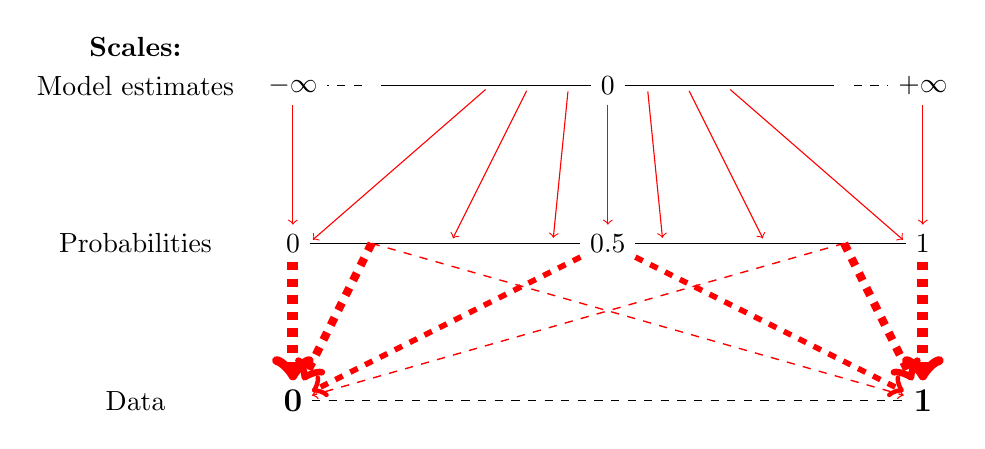
\begin{tikzpicture}
\node (sc) at (-6, 0.5) {\textbf{Scales:}};
\uncover<2->{
  \node (mininf) at (-4,0) {$- \infty $};
  \node (maxinf) at (4,0) {$+ \infty $};
  \node (binf) at (-3,0) {};
  \node (tinf) at (3,0) {};
  \node (zer) at (0,0) {$0$};
  \draw (binf) -- (zer) -- (tinf);
  \draw[dashed] (binf)--(mininf);
  \draw[dashed] (tinf)--(maxinf);
  \node (modest) at (-6,0) {Model estimates};
}
\uncover<3->{
  \node (prb) at (-6,-2) {Probabilities};
  \node (minpr) at (-4,-2) {0};
  \node (maxpr) at (4,-2) {1};
  \node (zerp) at (0,-2) {$0.5$};
  \draw (minpr)-- (zerp) -- (maxpr);
}
\uncover<4->{
  \node (dat) at (-6,-4) {Data};
  \node (mind) at (-4,-4) {\large \textbf{0}};
  \node (maxd) at (4,-4) {\large \textbf{1}};
  \draw[dashed] (mind)--(maxd);
}

\uncover<5->{

\draw[->, draw=red] (zer) -- (zerp);
\draw[->, draw=red] (mininf) -- (minpr);
\draw[->, draw=red] (maxinf) -- (maxpr);

\draw[->, draw=red, shorten <= 2pt, shorten >= 2pt] (-0.5,0) -- (-0.7,-2);
\draw[->, draw=red, shorten <= 2pt, shorten >= 2pt] (0.5,0) -- (0.7,-2);

\draw[->, draw=red, shorten <= 2pt, shorten >= 2pt] (-1,0) -- (-2,-2);
\draw[->, draw=red, shorten <= 2pt, shorten >= 2pt] (1,0) -- (2,-2);


\draw[->, draw=red, shorten <= 2pt, shorten >= 2pt] (-1.5,0) -- (-3.8,-2);
\draw[->, draw=red, shorten <= 2pt, shorten >= 2pt] (1.5,0) -- (3.8,-2);

}

\uncover<6->{
\draw[->, draw=red, dashed, line width=2pt] (zerp) -- (mind);
\draw[->, draw=red, dashed, line width=2pt] (zerp) -- (maxd);

\draw[->, draw=red, dashed, line width=4pt] (minpr) -- (mind);
\draw[->, draw=red, dashed, line width=4pt] (maxpr) -- (maxd);

\draw[->, draw=red, dashed, line width=3pt] (-3,-2) -- (mind);
\draw[->, draw=red, dashed, line width=0.5pt] (-3,-2) -- (maxd);

\draw[->, draw=red, dashed, line width=3pt] (3,-2) -- (maxd);
\draw[->, draw=red, dashed, line width=0.5pt] (3,-2) -- (mind);
}
\end{tikzpicture}
\end{center}

\uncover<7->{
\begin{block}{Conversion:}
\begin{itemize}
  \item from model to probability: $p=\frac{1}{1+\exp(-x)}$ or \texttt{plogis(x)}
  \item probability and data on same scale, but continuous/discrete
  \item $\exp(slope)$ = odd-ratio
\end{itemize}
\end{block}
}
\end{frame}
%%%%%%%%%%%%%%%%%%%%%%%

\begin{frame}{Exercise 3, interpretation}


\end{frame}
%%%%%%%%%%%%%%%%%%%%%%
\begin{frame}{Exercise 4, visualize model}


\end{frame}
%%%%%%%%%%%%%%%%%%%%%%

\begin{frame}{Take pictures!}
BDSI would like some pictures to illustrate their website. Is everybody okay with pictures?
\end{frame}
%%%%%%%%%%%%%%%%%%%%%%%

\begin{frame}{Clustering}

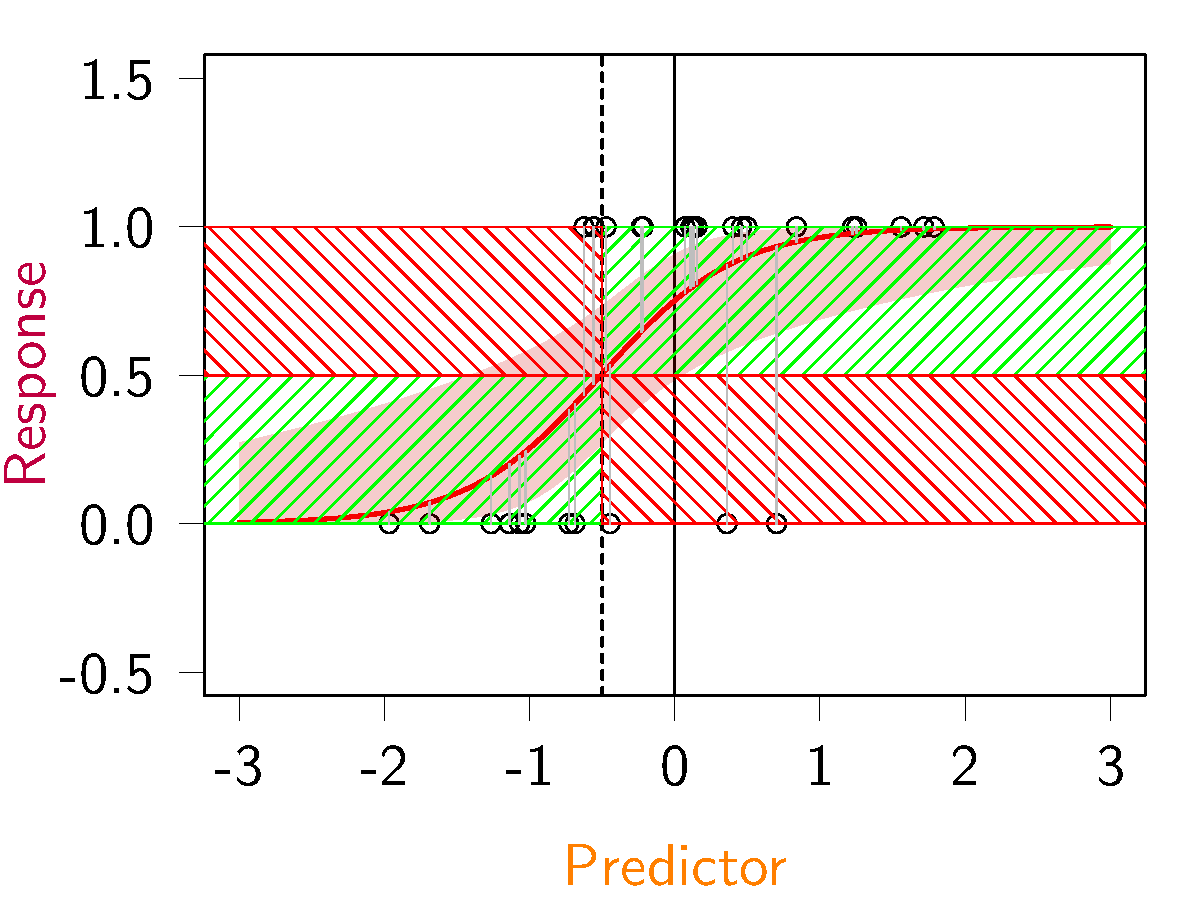
\includegraphics[width=0.8\textwidth]{figure/logreg3-1}

\end{frame}
%%%%%%%%%%%%%%%%%%%%%%

\begin{frame}{Clustering: what threshold?}
\centering
\only<1>{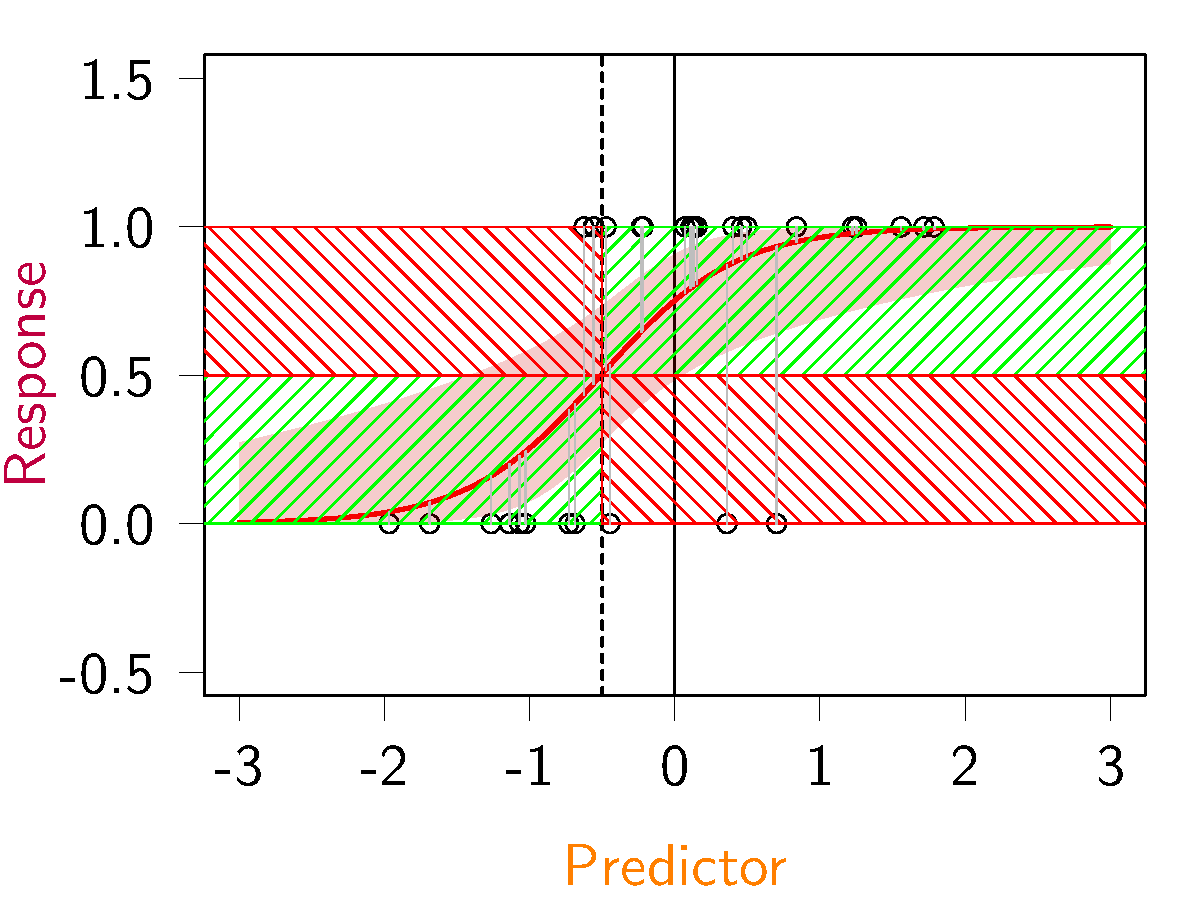
\includegraphics[width=0.5\textwidth]{figure/logreg3-1}}

\only<2>{
\begin{knitrout}\small
\definecolor{shadecolor}{rgb}{0.843, 0.867, 0.922}\color{fgcolor}

{\centering 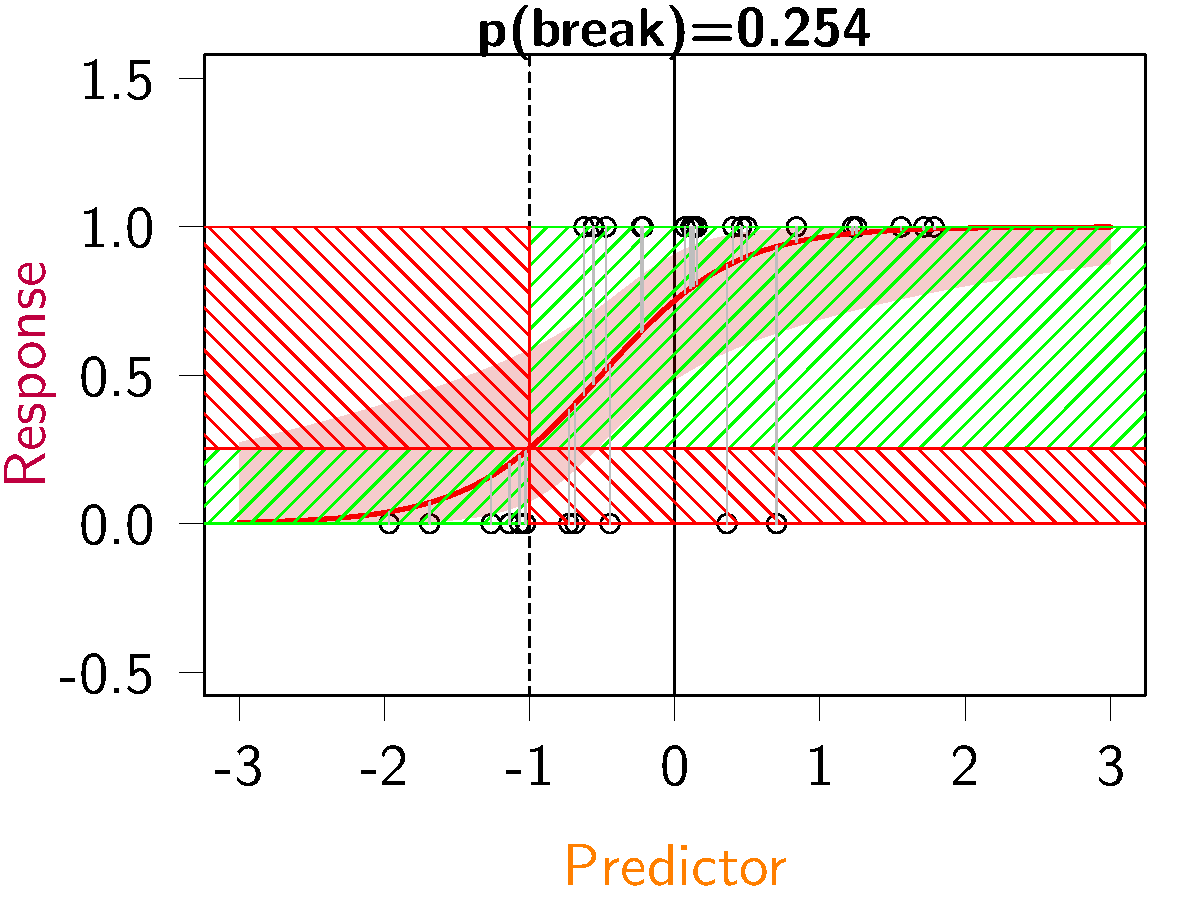
\includegraphics[width=0.5\textwidth,height=0.5\textheight]{figure/logreg4-1} 

}



\end{knitrout}
}

\only<3>{
\begin{knitrout}\small
\definecolor{shadecolor}{rgb}{0.843, 0.867, 0.922}\color{fgcolor}

{\centering 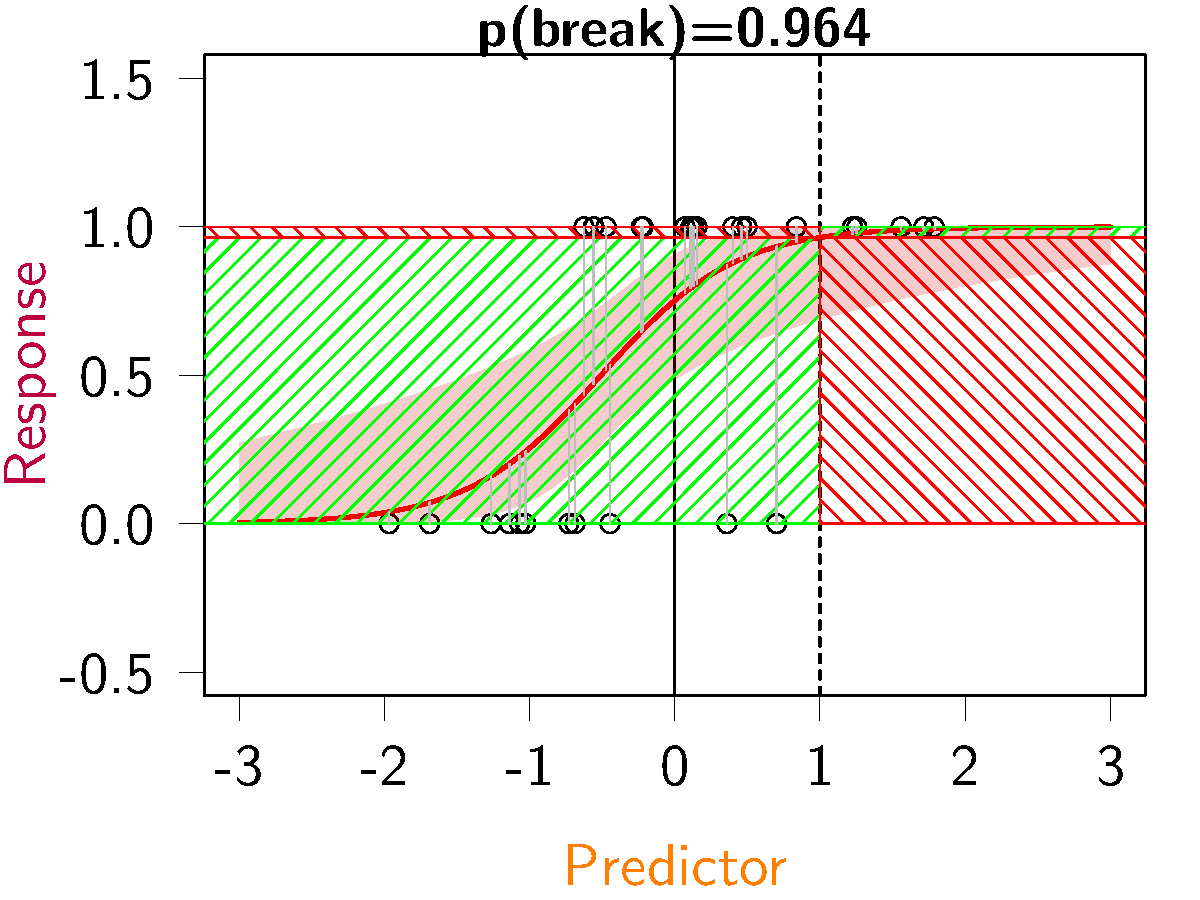
\includegraphics[width=0.5\textwidth,height=0.5\textheight]{figure/logreg5-1} 

}



\end{knitrout}
}
\begin{block}{}
\begin{itemize}[<+->]
  \item Break at 50\% probability?
  \item Never miss a case? (but false positives!) e.g., Epidemic prevention
  \item Never false positive? (but miss some positives!) e.g., Presumption of innocence
\end{itemize}
\end{block}

\end{frame}
%%%%%%%%%%%%%%%%%%%%%%%%%
 
 \begin{frame}{Exercise 5 }
 
 \pause
 
 \begin{exampleblock}{How good is the classification? What threshold to use?}
   \begin{itemize}
     \item Receiver Operating Characteristic and Area Under the Curve (ROC / AUC)
     \item E.g., \texttt{library(pROC)}
   \end{itemize}
   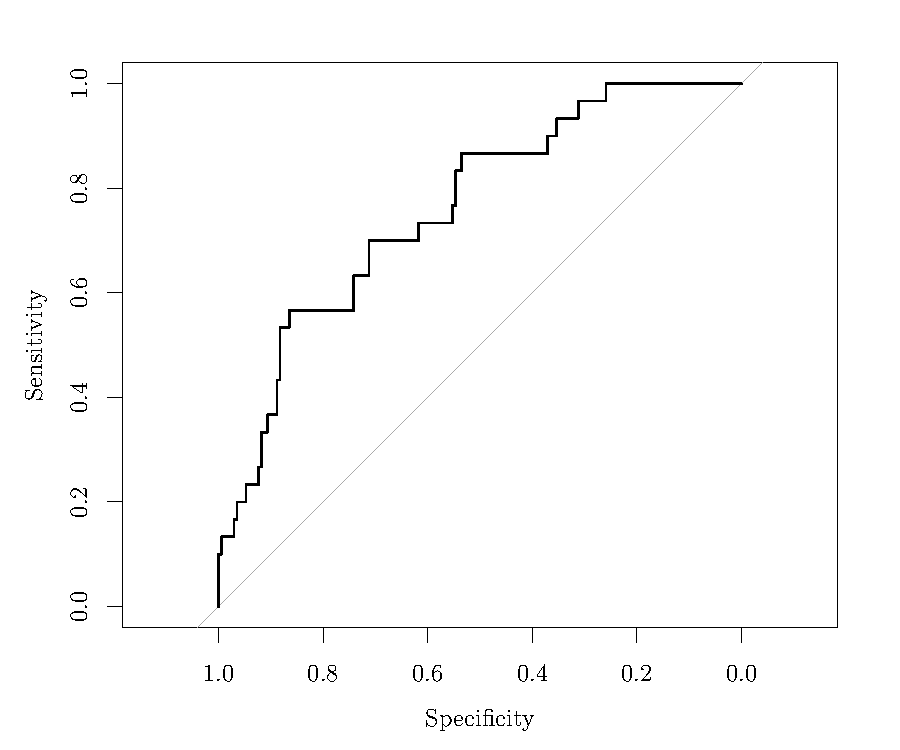
\includegraphics[width=0.3\textwidth]{figure/rocplot-1}
 \end{exampleblock}
%
 \end{frame}
%%%%%%%%%%%%%%%%%%%%%%%


\begin{frame}[fragile]{Mixed effect logistic regression}
GLM + random effect = GLMM\\
\pause
\begin{knitrout}\small
\definecolor{shadecolor}{rgb}{0.843, 0.867, 0.922}\color{fgcolor}\begin{kframe}
\begin{alltt}
\hlkwd{library}\hlstd{(lme4)}
\hlkwd{glmer}\hlstd{(response} \hlopt{~} \hlnum{1} \hlopt{+} \hlstd{predictor} \hlopt{+} \hlstd{(}\hlnum{1}\hlopt{|}\hlstd{group),} \hlkwc{family}\hlstd{=}\hlstr{"binomial"}\hlstd{,}
          \hlkwc{data}\hlstd{=dat)}
\end{alltt}
\end{kframe}
\end{knitrout}

\end{frame}
%%%%%%%%%%%%%%%%%%%%%%%


\begin{frame}{Mixed effect logistic regression}
\begin{columns}
\begin{column}{0.3\textwidth}
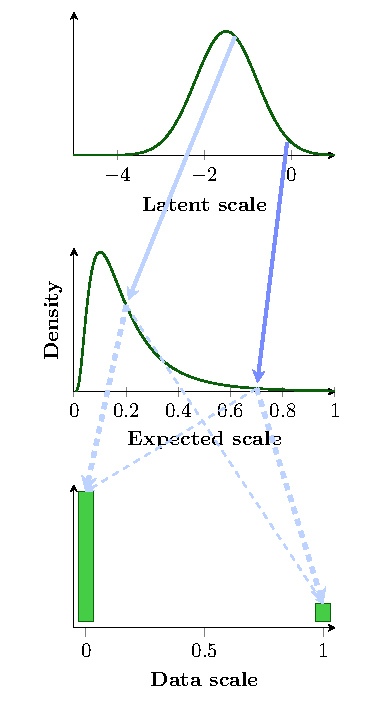
\includegraphics[height=0.8\textheight]{figure/backtransformation.pdf}
\end{column}
\begin{column}{0.7\textwidth}
\begin{itemize}
  \item There is no meaningful residual variance
  \item Random effect variance distorted by logit
  \item Lots of variance from random process on top of expected values
\end{itemize}
\end{column}
\end{columns}

\end{frame}
%%%%%%%%%%%%%%%%%%%%%

\begin{frame}{Repeatability in GLMM}

In LMM: repeatability = variance random effect / (variance random effect + residual variance)\\

\pause

\begin{alertblock}{but in GLMM, especially logistic:}
\begin{itemize}
  \item On what scale to take the random effect?
  \item No residual variance! Is repeatability always 1??
\end{itemize}
\end{alertblock}

\vfill

\textbf{Exercise 6}

\end{frame}
%%%%%%%%%%%%%%%%%%%%%%%
\end{document}
